
\chapter{Introduction}
The primary content of my thesis is the four papers that are included in the thesis. This chapter is meant as a brief introduction to the background needed to understand the basics of the methods used throughout the papers. As such, this chapter is not meant to be a comprehensive guide to statistics and bioinformatics used in the papers. The original research motivation supporting the funding of this Ph.D. was very multi-disciplinary and the papers included in my thesis are also clearly influenced by this.

In \autoref{section:ancientDNA}, I will shortly introduce the field of ancient genomics and the statistical methods used to identify ancient DNA will be explained. Paper I, see \autoref{chapter:metadmg}, utilize modern Bayesian methods to classify which species are ancient and which ones are not. Bayesian methods are great when possible, however, they also rely on some statistical model being defined. In the case of Paper I, the model is a Beta-Binomial distribution combined with an exponential-decay damage model.

Sometimes, however, the model is not known and the data generating process has to be inferred by other means. This is the case in Paper II, see \autoref{chapter:hospital}, where we utilize machine learning methods to extract this information. This paper deals with estimating the individual risk scores for each patient being re-hospitalized after a knee or hip operation. \autoref{section:machine-learning} introduces the reader to basic classification with machine learning models.

While the former two papers are based on real life data, Paper III, see \autoref{chapter:covid19-agent-based-model}, concerns the development of a new agent based model for COVID-19. The model is based on the SIR model, but with a more detailed description of the disease and the transmission process. The model is used to simulate the spread of the virus in Denmark and to estimate the effect of contact tracing. The model is also used to simulate and predict the spread of the ``alpha'' variant of COVID-19 in Denmark. \autoref{section:agent-based-models} introduces the reader to the basics of agent based models.

Finally, the method of Bayesian model comparison of different diffusion models is introduced in Paper IV, see \autoref{chapter:diffusion}. In particular, this paper deals with different mixture-models of independent Rayleigh-distributions and how they can be used to extract important information about the underlying diffusion processes of a polymer bridging model in cell nuclei, see \autoref{section:diffusion}.

\section{Ancient DNA and Bayesian Statistics}
\label{section:ancientDNA}

Previously, the only way to study ancient animals, plants, and other species was by studying their fossils. This changed in the middle of the 1980's when the first DNA was recovered from almost 5000 years old ancient mummies, showing that it was indeed possible to extract and sequence ancient DNA \autocite{paaboMolecularCloningAncient1985,paaboPreservationDNAAncient1985}. This discovery, along with a dozen other pushing the boundary for what is scientifically possible with ancient DNA, led to Svante Pääbo being awarded with the Nobel Prize in Physiology or Medicine in 2022 for ``his discoveries concerning the genomes of extinct hominins and human evolution'' \autocite{thenobelassemblyatkarolinskainstitutetNobelPrizePhysiology2022}.

The field of ancient DNA (aDNA) was drastically changed with the invention of the Polymerase Chain Reaction, PCR, method \autocite{mullisSpecificEnzymaticAmplification1986} along with the Next Generation Sequencing technology which revolutionized the speed and throughput of genomic sequencing while decimating the cost \autocite{slatkoOverviewNextGeneration2018}. This technological advance has lead to better understanding of human migration and the genealogical tree of modern humans including the previously unknown human (sub)species; the Denisova hominin \autocite{krauseCompleteMitochondrialDNA2010}.

Leaving the homocentric world view, aDNA also allows for the study of archaic animals. In recent years, the boundary of how old DNA can be sequenced has been severely pushed; in 2013 with the early Middle Pleistocene \qtyrange[range-phrase = --,range-units = single]{560}{780}{\kilo\year\BP} horse \autocite{orlandoRecalibratingEquusEvolution2013} and in 2021 with the million-year-old mammoths \autocite{vandervalkMillionyearoldDNASheds2021}. High-throughput sequencing not only allows for the sequencing of single genomes -- like single humans, animals, or plants -- but also for sequencing of entire communities of organisms, so-called metagenomics. By analysing the DNA in environmental samples, environmental DNA, one can survey the rich plant and animal assemblages of a given area and at a specific time in the past. A new paper published in Nature shows that it is now possible to perform metagenomic sequencing on environmental DNA that is 2 million years old, see \autoref{appendix:kapk}. This is a direct application of the statistical method developed in Paper I, see \autoref{chapter:metadmg}, showing that \metaDMG, the method, can help to push the boundary of what is possible with ancient DNA.

Ancient DNA is difficult to work with since it often contains only a limited amount of biological material due to bad preservation, leading to low endogenous content with high duplication rates, making high-depth sequencing difficult \autocite{renaudAuthenticationAssessmentContamination2019}. Genotype likelihoods are often used to alleviate the problem of low-coverage data \autocite{nielsenGenotypeSNPCalling2011}.
In addition to this, the DNA is often highly degraded. In particular, the two prominent issues with aDNA is fragmentation and deamination \autocite{dabneyAncientDNADamage2013,peyregnePresentDayDNAContamination2020,}. Fragmentation refers to the fact that the DNA is broken into very short fragments, often with a fragment size of less than \SI{50}{\basepairs}. This leads to low-quality mapping issues and reference biases, which can somewhat be mitigated by the use variant graphs \autocite{martinianoRemovingReferenceBias2020}.
Deamination is a process in which cytosine (C) in the single-stranded overhangs in the end of the DNA molecules is often hydrolized to uracil (U) which is then read as thymine (T) by the DNA polymerase. This particular type of postmortem damage is known as cytosine deamination, or C-to-T transitions, and is a one of the main reasons behind nucleotide misincorporations in ancient DNA \autocite{briggsPatternsDamageGenomic2007}. Due to the short fragment sizes in ancient DNA, they will often contain overhangs with over-expressed C-to-T frequency. In the case of single-genome analysis, previous solutions have been to either remove all transitions and only keep transversions, or apply trimming at the read ends \autocite{schubertImprovingAncientDNA2012}.
For an illustration of both fragmentation and deamination of ancient DNA, see  \autoref{fig:dna-damage-overview}.

\begin{figure}[htbp]
    \sidecaption{
        Illustration of DNA damage. Ancient DNA is often highly fragmented with short reads compared to modern, present-day DNA, and can contain uracils (U). These uracils will then be misread as thymines (T) while sequencing leading to C-T nucleotide misincorporations. This is primaryly happening at the end of the reads. Modified from \autocite{peyregnePresentDayDNAContamination2020}.
        \label{fig:dna-damage-overview}}
    \centering
    \includegraphics[trim={0mm 90mm 0mm 90mm}, clip, width=\textwidth]{figures/illustrator/dna-deamination.pdf}
\end{figure}

Currently, a handfull of different methods for quantifying ancient DNA damage exists. In particular, the mapDamage 2.0 software has been the gold standard for how to measure ancient DNA damage in the field \autocite{jonssonMapDamage2FastApproximate2013}, however, it uses slow algorithms leading to unfeasible runtimes for large datasets. Newer, faster methods are being developed all of the time, such as PyDamage \autocite{borryPyDamageAutomatedAncient2021} which tackle some of mapDamage's limitations, although even faster methods suited at metagenomic analysis for large-scale datasets are still lacking.

In Paper I, see \autoref{chapter:metadmg}, we introduce the \metaDMG  software which utilizes the C-to-T deamination pattern\sidenote{for the forward strand and the G-to-A deamination pattern for the reverse strand} to identify ancient DNA damage. One of the key features of this method is the beta-binomial model which allows the uncertainty to fitted independently of the mean leading to improved accuracy of the damage estimation. Since the data is based on misincorporation counts, in particular the number of C-to-T transitions, $k$, out of $N$ total C's, the classical likelihood  to use for this type of data is a binomial distribution. The mean and variance of the binomial distribution is given by:
\begin{equation}
    \begin{split}
        \EX{k}  &= N \mu \\
        \VarX{k} &= N\mu(1-\mu) \frac{\phi+N}{\phi+1}.
        \label{eq:P_BetaBinom_expectation_variance}
    \end{split}
\end{equation}


\begin{figure}[htbp]
    \sidecaption{
        Illustration of the damage model. The figure shows data points as circles and the damage, $f(x)$, as a solid line. The amplitude of the damage is $A$, the offset is $c$, and the relative decrease in damage pr. position is given by $q$. The damage uncertainty for a binomial model is shown in dark grey and the uncertainty for a beta-binomial model in light grey.
        \label{fig:damage-model-sketch}}
    \centering
    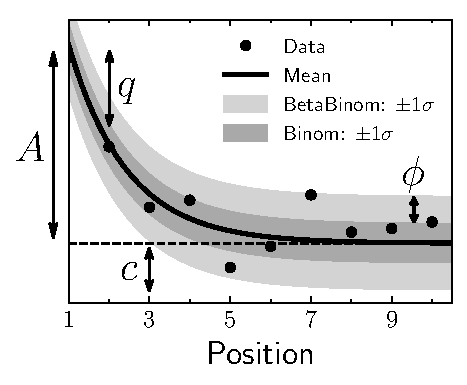
\includegraphics[width=0.6\textwidth]{figures/damage_sketch.pdf}
\end{figure}




\section{Anestesiology -- a Machine Learning Approach }
\label{section:machine-learning}

asdasdasd


\section{COVID-19 and Agent Based Models}
\label{section:agent-based-models}
asdasdasdads

\section{Diffusion Models and Bayesian Model Comparison}
\label{section:diffusion}
asdasdas
